\section{Die Implementierung}

\subsection{Das Programm}

\subsection{Simulations-Ergebnisse}

\subsubsection{Der kritische Punkt}

\subsubsection{Domänenwände beim Antiferromagneten}
Bei geringen Temperaturen gibt es in einem Antiferromagneten nur noch sehr wenige Störstellen.
Da sich das \textit{Schachbrettmuster} beim Abkühlen von mehreren Stellen gleichzeitig ausbreitet, bleiben am Ende einige Stellen übrig, an denen es unterbrochen ist. Diese Domänenwände haben eine Breite von genau zwei Spins, die nebeneinander die gleiche Ausrichtung haben.
Es wäre energetisch viel aufwändiger, einen ganzen Bereich mit \textit{falscher} Ausrichtung umzudrehen, als diese dünnen Wände stehen zu lassen.

Obwohl die Simulation bei uns mit konstanter Temperatur abläuft, wird praktisch eine Abkühlung simuliert.
Die Startkonfiguration ist eine Zufallsverteilung, die einer hohen Temperatur entspricht.

\begin{figure}[h]
  \subfloat[Mittelwerte der Spins]{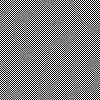
\includegraphics[width=200pt]{bilder/domainwall/beta_1.png}}
  \hfill
  \subfloat[Letzte Spin-Konfiguration der Messung]{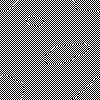
\includegraphics[width=200pt]{bilder/domainwall/spins_1.png}}
  \caption{Domänenwände eines Antiferromagneten bei $\beta\approx 345, J=-1, B=0$\label{domainwall}}
\end{figure}
Abbildung \ref{domainwall} zeigt eine Beispielsimulation, bei der Domänenwände sichtbar werden.
Simuliert wurde in zwei Dimensionen mit $100^2$ Spins und ohne externes Magnetfeld.
Die Simulation ist nur eingeschränkt auf die Realität übertragbar, da die Grundannahme des Ising-Modells, dass Spins nur in einer Achse ausgerichtet sein können, ohne externes Magnetfeld natürlich nicht erfüllt ist.

Bei den Abbildungen weichen die Mittelwerte doch an einigen Stellen deutlich von der Momentaufnahme ab.
Um hier wirklich ein statisches Bild zu geben, scheint die Temperatur noch nicht niedrig genug zu sein.

\subsubsection{Hysterese beim Ferromagneten}
Ein Ferromagnet widersteht einem wechselnden äußeren Magnetfeld, bevor er selbst seine Ausrichtung ändert.
Diese Hysterese lässt sich auch mit dem Ising-Modell gut beschreiben.

\begin{wrapfigure}{r}{8.5cm}
  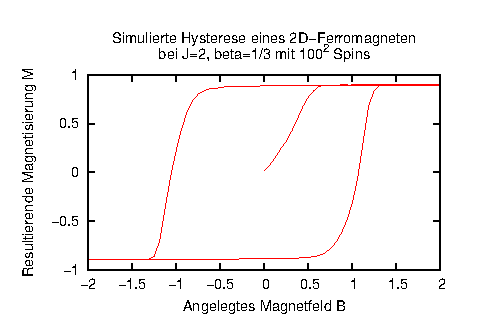
\includegraphics[width=0.6\textwidth]{bilder/hysterese/hysterese.eps}
  \caption{Hysterese eines Ferromagneten. Die Simulation ging mit 400 Schritten: $B=0\to 5 \to -5 \to 5$\label{hysterese}}
\end{wrapfigure}
Für die Simulation haben wir wieder $100^2$ Spins mit einer ferromagnetischen Wechselwirkung von $J=2$.
Die Temperatur ist mit $\beta=\frac 13$ klein genug für die ferromagnetische Phase.
Das externe Magnetfeld läuft von $B=0$ bis zur Sättigung $B=5$, anschließend bis $B=-5$ und noch einmal ins Positive.
Dabei wird $B$ in 400 Einzelschritten linear geändert und mit jeweils $10^5$ Monte-Carlo-Schritten stabilisiert.
Das Ergebnis (Abbildung \ref{hysterese}) zeigt einen relativ glatten Verlauf und die Rechenzeit hielt sich mit 21 Sekunden in Grenzen, so dass wir bislang keine weitere Geschwindigkeitsoptimierung vorgenommen haben.

\begin{figure}[h]
    \subfloat{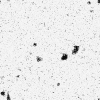
\includegraphics[width=0.15\textwidth]{bilder/hysterese/b_169.png}}
  \hfill
    \subfloat{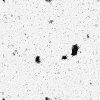
\includegraphics[width=0.15\textwidth]{bilder/hysterese/b_170.png}}
  \hfill
    \subfloat{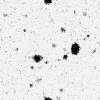
\includegraphics[width=0.15\textwidth]{bilder/hysterese/b_171.png}}
  \hfill
    \subfloat{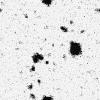
\includegraphics[width=0.15\textwidth]{bilder/hysterese/b_172.png}}
  \hfill
    \subfloat{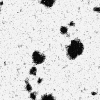
\includegraphics[width=0.15\textwidth]{bilder/hysterese/b_173.png}}
  \hfill
    \subfloat{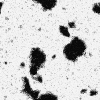
\includegraphics[width=0.15\textwidth]{bilder/hysterese/b_174.png}}
  \\
    \subfloat{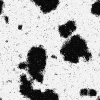
\includegraphics[width=0.15\textwidth]{bilder/hysterese/b_175.png}}
  \hfill
    \subfloat{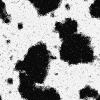
\includegraphics[width=0.15\textwidth]{bilder/hysterese/b_176.png}}
  \hfill
    \subfloat{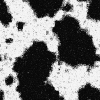
\includegraphics[width=0.15\textwidth]{bilder/hysterese/b_177.png}}
  \hfill
    \subfloat{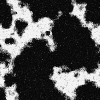
\includegraphics[width=0.15\textwidth]{bilder/hysterese/b_178.png}}
  \hfill
    \subfloat{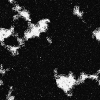
\includegraphics[width=0.15\textwidth]{bilder/hysterese/b_179.png}}
  \hfill
    \subfloat{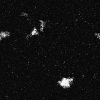
\includegraphics[width=0.15\textwidth]{bilder/hysterese/b_180.png}}
\caption{Ausrichtungswahrscheinlichkeiten der Spins beim Richtungswechsel der Hysteresekurve.\label{hysterese-wechsel}}
\end{figure}

Der Übergang von positiver zu negativer Magnetisierung der Hysteresekurve ist nochmal in Bildern in Abbildung \ref{hysterese-wechsel} zu sehen.
Hier sind die Mittelwerte der einzelnen Spins (ein Spin pro Pixel) wie in Abbildung \ref{domainwall} (a) zu sehen.
Man kann gut die zufälligen Strukturen erkennen, die sich beim Übergang ergeben.
Bestehende Flächen von Spins, die schon negativ (schwarz) ausgerichtet sind, werden immer größer und breiten sich immer weiter aus.

